\documentclass[]{standalone}
\usepackage[dvipsnames]{xcolor}
\usepackage{tikz-network}
\begin{document}
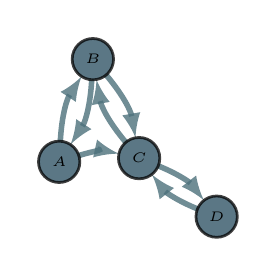
\begin{tikzpicture}
    \pgfmathsetmacro{\width}{2.0}
    \pgfmathsetmacro{\height}{2.0}
    \pgfmathsetmacro{\margin}{0.5 + 0.2}
    \tikzset{every node}=[font=\sffamily\bfseries]
    \clip (-\margin*\width cm,-\margin*\height cm) rectangle (\margin*\width cm,\margin*\height cm);
    \draw[draw,opacity=0] (-\margin*\width cm,-\margin*\height cm) rectangle (\margin*\width cm,\margin*\height cm);
    \Vertex[label=$A$,fontsize=\fontsize{4}{10}\selectfont,RGB,color={36, 74, 92},size=0.525,opacity=0.75,style={draw opacity=0.75},x=-1.0,y=-0.3038503]{A};
\Vertex[label=$B$,fontsize=\fontsize{4}{10}\selectfont,RGB,color={36, 74, 92},size=0.525,opacity=0.75,style={draw opacity=0.75},x=-0.57189626,y=1.0]{B};
\Vertex[label=$C$,fontsize=\fontsize{4}{10}\selectfont,RGB,color={36, 74, 92},size=0.525,opacity=0.75,style={draw opacity=0.75},x=0.015314817,y=-0.25673693]{C};
\Vertex[label=$D$,fontsize=\fontsize{4}{10}\selectfont,RGB,color={36, 74, 92},size=0.525,opacity=0.75,style={draw opacity=0.75},x=1.0,y=-1.0]{D};
\Edge[bend=15,Direct,RGB,color={76, 112, 123},lw=2,opacity=0.8](A)(B);
\Edge[bend=15,Direct,RGB,color={76, 112, 123},lw=2,opacity=0.8](A)(C);
\Edge[bend=15,Direct,RGB,color={76, 112, 123},lw=2,opacity=0.8](B)(C);
\Edge[bend=15,Direct,RGB,color={76, 112, 123},lw=2,opacity=0.8](B)(A);
\Edge[bend=15,Direct,RGB,color={76, 112, 123},lw=2,opacity=0.8](C)(D);
\Edge[bend=15,Direct,RGB,color={76, 112, 123},lw=2,opacity=0.8](C)(B);
\Edge[bend=15,Direct,RGB,color={76, 112, 123},lw=2,opacity=0.8](D)(C);

\end{tikzpicture}
\end{document}
